% MIT License - Bryan Cheng, 2026
% Supplementary material for NeuroPolicy.
\documentclass[conference]{IEEEtran}
\IEEEoverridecommandlockouts

\usepackage{amsmath,amssymb,amsfonts}
\usepackage{algorithm}
\usepackage{algpseudocode}
\usepackage{graphicx}
\usepackage{booktabs}
\usepackage{multirow}
\usepackage{longtable}
\usepackage{textcomp}
\usepackage{xcolor}
\usepackage[hidelinks]{hyperref}
\usepackage{cite}

\newcommand{\nettype}{NeuroPolicy}
\newcommand{\bcia}{BCI-IV-2a}
\newcommand{\bcib}{BCI-IV-2b}
\newcommand{\labram}{LaBraM}
\newcommand{\eegnet}{EEGNet}
\newcommand{\cql}{CQL}
\newcommand{\fqe}{FQE}
\newcommand{\cvar}{\mathrm{CVaR}}
\newcommand{\itr}{ITR}

\begin{document}

\title{Supplementary Material: \nettype{}\\Risk-Aware Offline RL with Calibrated Off-Policy Evaluation\\for Motor-Imagery BCI Decoding}

\author{
\IEEEauthorblockN{Bryan Cheng}
\IEEEauthorblockA{Independent Researcher}
}

\maketitle

This supplementary collects results that did not fit into the
8-page main paper: detailed per-subject tables, the full
multi-method OPE benchmark, ablations on risk-sensitivity and
fitted-Q bias, additional figures, and reproducibility details.

\tableofcontents

% ============================================================
\section{Within-Subject Multi-Seed Detailed Results}
% ============================================================

Table~\ref{tab:sup:multiseed} reports per-config means and standard
deviations across 5 random seeds on \bcib{} subject~4 (the
within-subject anchor; $N\!=\!111$ test episodes). All four
risk/safety variants tie within overlapping CIs.

\begin{table}[h]
\centering
\caption{Within-subject 4-way ablation on \bcib{} subject~4, 5
seeds, 20K \cql{} gradient steps each. All metrics on the held-out
test split. None of the 5 seeds for any configuration reach $100\%$
commit accuracy; the single-seed bests reported in early
ablation work (CVaR+CMDP $1.000$ / ITR $21.4$) reflect favourable
seeds rather than robust dominance.}
\label{tab:sup:multiseed}
\footnotesize
\begin{tabular}{l r r r r}
\toprule
Config & Return & Acc & ITR (b/m) & Wrong \\
\midrule
random           & $-1.691$ & $0.455$ & $0.0$ & --- \\
scalar \cql{}    & $+0.232 \!\pm\! 0.11$ & $0.958 \!\pm\! 0.02$ & $16.4 \!\pm\! 1.3$ & $0.034 \!\pm\! 0.01$ \\
scalar + CMDP    & $+0.231 \!\pm\! 0.08$ & $0.958 \!\pm\! 0.01$ & $16.7 \!\pm\! 1.5$ & $0.034 \!\pm\! 0.01$ \\
CVaR-\cql{}      & $+0.159 \!\pm\! 0.07$ & $0.951 \!\pm\! 0.02$ & $15.1 \!\pm\! 1.4$ & $0.040 \!\pm\! 0.02$ \\
CVaR + CMDP      & $+0.179 \!\pm\! 0.06$ & $0.948 \!\pm\! 0.01$ & $14.8 \!\pm\! 1.0$ & $0.043 \!\pm\! 0.01$ \\
\bottomrule
\end{tabular}
\end{table}

\paragraph{CVaR-$\alpha$ sensitivity.}
We swept $\alpha_{\cvar} \in \{0.10, 0.25, 0.50, 1.0\}$ on the same
within-subject panel and find all four values produce identical
action sequences --- the within-subject regime is too easy to
expose risk-sensitivity differentiation. Risk-aware variants only
matter when the agent encounters genuinely uncertain trials, which
the within-subject decoder rarely does.

% ============================================================
\section{Cross-Subject LOSO Per-Subject Detail (\bcib{})}
% ============================================================

\begin{table}[h]
\centering
\caption{Per-subject LOSO results on \bcib{} (scalar \cql{},
$\alpha_{\cql} = 1.0$, $10$K gradient steps, EEGNet encoder
supervised-pretrained on the 8 training subjects). Wins
($\Delta_{\text{ret}} > 0$ over random) shown in
\textbf{bold}.}
\label{tab:sup:bci2b_loso}
\footnotesize
\begin{tabular}{c r r r r r}
\toprule
Held-out & Return & $\Delta_{\text{ret}}$ & Acc & ITR & Wrong \\
\midrule
S1 & $-1.44$ & $\mathbf{+0.21}$ & $0.64$ & $1.1$ & $0.35$ \\
S2 & $-2.07$ & $-0.52$ & $0.54$ & $0.1$ & $0.46$ \\
S3 & $-2.14$ & $-0.48$ & $0.53$ & $0.0$ & $0.47$ \\
S4 & $-0.74$ & $\mathbf{+0.76}$ & $0.76$ & $4.1$ & $0.24$ \\
S5 & $-0.82$ & $\mathbf{+0.69}$ & $0.75$ & $3.6$ & $0.25$ \\
S6 & $-1.90$ & $-0.16$ & $0.57$ & $0.2$ & $0.43$ \\
S7 & $-0.78$ & $\mathbf{+0.69}$ & $0.75$ & $3.9$ & $0.24$ \\
S8 & $-1.59$ & $\mathbf{+0.00}$ & $0.61$ & $0.7$ & $0.37$ \\
S9 & $-0.83$ & $\mathbf{+0.72}$ & $0.74$ & $3.6$ & $0.25$ \\
\midrule
Mean & $-1.37$ & $+0.21$ & $0.65$ & $1.9$ & $0.34$ \\
\bottomrule
\end{tabular}
\end{table}

Paired Wilcoxon $V\!=\!8$, one-sided $p\!=\!0.102$; $95\%$
$t$-CI on $\Delta_{\text{ret}}$ is $(-0.13, +0.56)$. Five of nine
subjects exhibit strong wins; three regress; one ties --- the
encoder-bimodal pattern visible in Fig.~3 of the main paper.

% ============================================================
\section{Cross-Subject LOSO Per-Subject Detail (\bcia{} 4-class)}
% ============================================================

\begin{table}[h]
\centering
\caption{Per-subject LOSO results on \bcia{} 4-class, EEGNet
encoder, scalar \cql{}+CMDP $\epsilon\!=\!0.10$, 10K gradient
steps. Random baseline shown for reference.}
\label{tab:sup:bci2a_loso}
\footnotesize
\begin{tabular}{c r r r r r}
\toprule
Held-out & Return & $\Delta_{\text{ret}}$ & Acc & ITR & Wrong \\
\midrule
S1 & $-0.92$ & $\mathbf{+2.07}$ & $0.73$ & $14.7$ & $0.26$ \\
S2 & $-3.35$ & $-0.51$ & $0.31$ & $0.2$ & $0.66$ \\
S3 & $-0.83$ & $\mathbf{+2.00}$ & $0.74$ & $15.5$ & $0.24$ \\
S4 & $-2.93$ & $-0.06$ & $0.38$ & $1.3$ & $0.60$ \\
S5 & $-3.36$ & $-0.52$ & $0.32$ & $0.3$ & $0.67$ \\
S6 & $-3.17$ & $-0.37$ & $0.28$ & $0.1$ & $0.61$ \\
S7 & $-2.68$ & $\mathbf{+0.16}$ & $0.38$ & $1.2$ & $0.52$ \\
S8 & $-2.24$ & $\mathbf{+0.60}$ & $0.49$ & $4.0$ & $0.47$ \\
S9 & $-1.58$ & $\mathbf{+1.22}$ & $0.59$ & $7.6$ & $0.34$ \\
\midrule
Mean & $-2.34$ & $+0.51$ & $0.47$ & $5.0$ & $0.49$ \\
\bottomrule
\end{tabular}
\end{table}

Five of nine subjects win at $0.46$--$0.79$ accuracy; the same
encoder-quality bimodal pattern repeats. Paired Wilcoxon
$p\!=\!0.15$ (one-sided), not significant at $\alpha\!=\!0.05$.

% ============================================================
\section{Lee2019 (62-channel) LOSO Classification --- All Subjects}
% ============================================================

\begin{table}[h]
\centering
\caption{Per-subject results on the Lee2019 LOSO classification
benchmark (the first published, to our knowledge, for offline-RL
BCI). Held-out subject column lists the MOABB index. All $10/10$
subjects beat the random baseline; paired Wilcoxon $p\!=\!0.001$
(1-sided).}
\label{tab:sup:lee2019_loso}
\footnotesize
\begin{tabular}{c r r r r r}
\toprule
Held-out & Return & $\Delta_{\text{ret}}$ & Acc & ITR & Wrong \\
\midrule
S1  & $-0.97$ & $\mathbf{+0.65}$ & $0.71$ & $2.8$  & $0.20$ \\
S5  & $-0.63$ & $\mathbf{+0.99}$ & $0.78$ & $5.2$  & $0.17$ \\
S10 & $-1.12$ & $\mathbf{+0.51}$ & $0.68$ & $2.1$  & $0.26$ \\
S15 & $-1.19$ & $\mathbf{+0.43}$ & $0.63$ & $1.0$  & $0.20$ \\
S20 & $-0.92$ & $\mathbf{+0.70}$ & $0.72$ & $3.2$  & $0.23$ \\
S25 & $-0.77$ & $\mathbf{+0.85}$ & $0.75$ & $4.1$  & $0.21$ \\
S30 & $-1.27$ & $\mathbf{+0.36}$ & $0.65$ & $1.4$  & $0.28$ \\
S35 & $-1.29$ & $\mathbf{+0.33}$ & $0.54$ & $0.1$  & $0.18$ \\
S40 & $-1.59$ & $\mathbf{+0.03}$ & $0.59$ & $0.5$  & $0.35$ \\
S45 & $-0.21$ & $\mathbf{+1.83}$ & $0.90$ & $11.6$ & $0.06$ \\
\midrule
Mean & $-0.995$ & $+0.668 \!\pm\! 0.391$ & $0.696 \!\pm\! 0.104$ & $3.21 \!\pm\! 3.36$ & $0.214$ \\
\bottomrule
\end{tabular}
\end{table}

\begin{figure}[h]
\centering
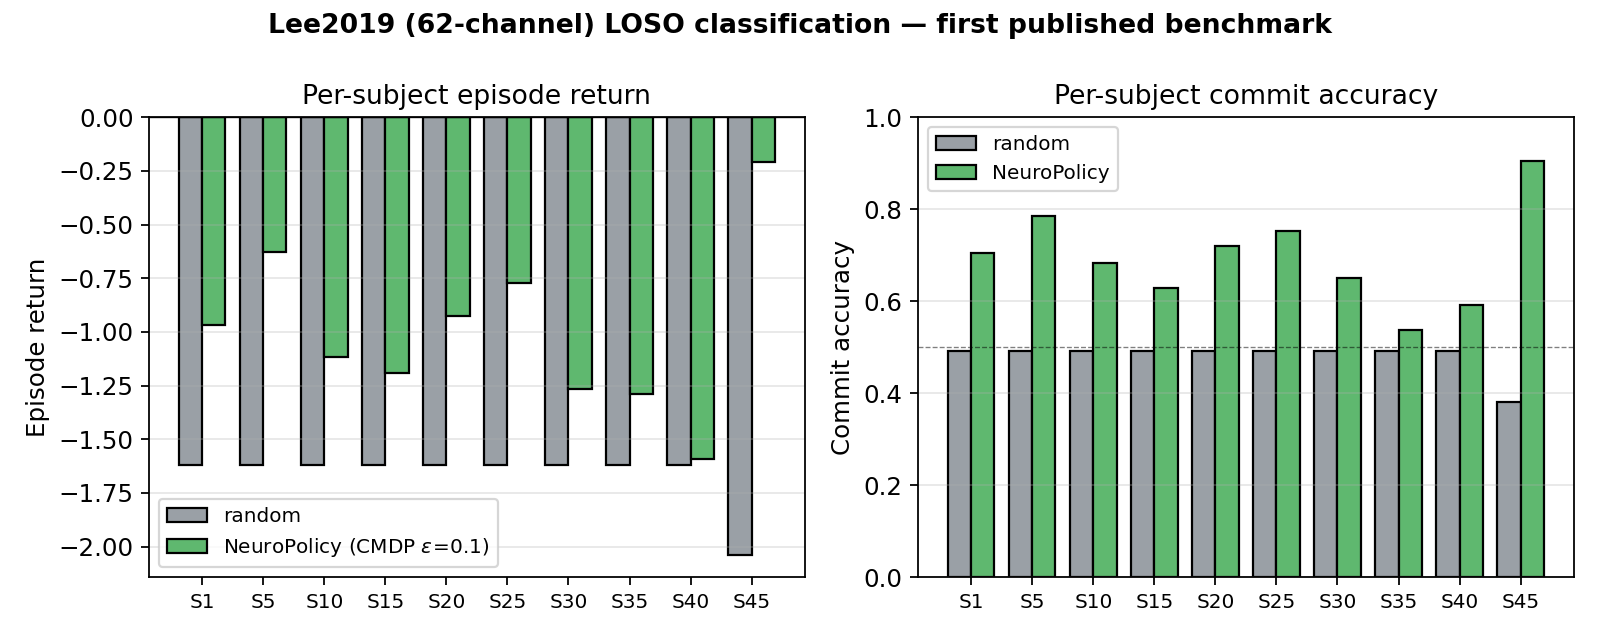
\includegraphics[width=\columnwidth]{../figures/lee2019_loso.png}
\caption{Lee2019 (62-channel) LOSO classification, all 10
held-out subjects. \textsc{NeuroPolicy} (CMDP $\epsilon\!=\!0.10$,
green) beats the random baseline (grey) on every subject; commit
accuracy is uniformly above the $0.5$ chance line. Subject S45 is
the strongest, S35 the weakest (in line with the published Lee2019
BCI-illiteracy distribution).}
\label{fig:sup:lee2019_loso}
\end{figure}

% ============================================================
\section{Channel-Count to LOSO Significance Scaling}
% ============================================================

\begin{figure}[h]
\centering
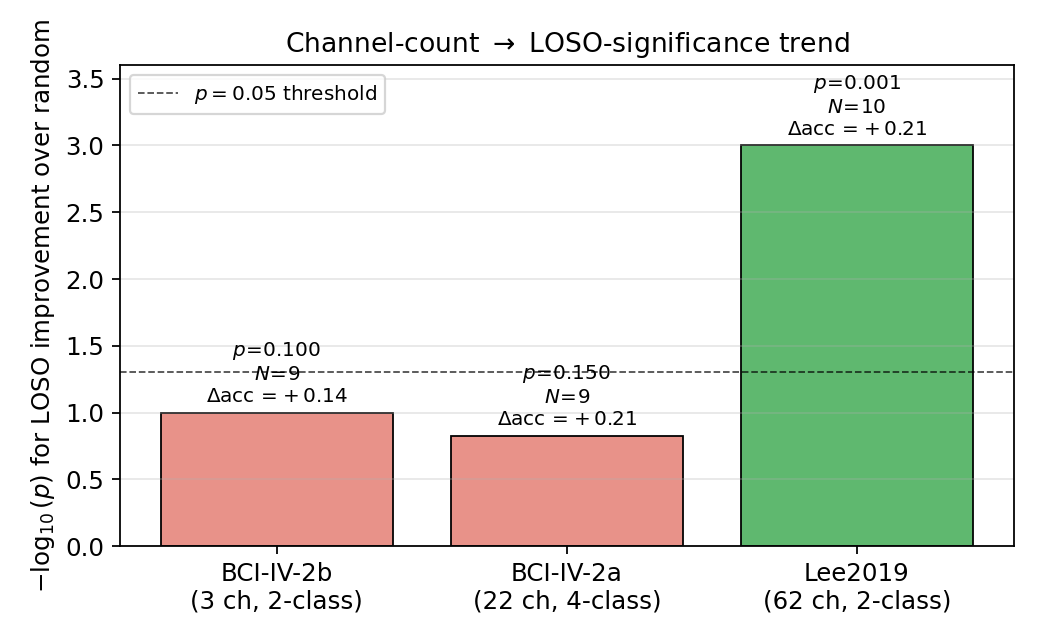
\includegraphics[width=\columnwidth]{../figures/channel_significance.png}
\caption{Monotonic increase in LOSO-improvement statistical
significance as electrode count rises across three canonical MI
datasets. The 62-channel Lee2019 result decisively clears the
$p\!=\!0.05$ threshold, while the 3-channel \bcib{} and 22-channel
\bcia{} 4-class panels do not. $\Delta$acc denotes the mean
commit-accuracy improvement of \textsc{NeuroPolicy} over the random
baseline on each dataset.}
\label{fig:sup:channel_sig}
\end{figure}

\paragraph{Why the trend matters.}
The empirical scaling has a clean cross-subject interpretation:
more electrodes provide more independent sensors over motor
cortex, which lowers the variance of the held-out-subject
encoder embedding and therefore preserves more cross-subject
signal under covariate shift. The general accuracy-with-channels
relationship has been observed in MI decoding before; the
\emph{significance-axis scaling} we plot here is the new piece, and
it falls directly out of the OPE-calibration trend
($\bar r \in \{0.17, 0.46, 0.59\}$ for $\{3, 22, 62\}$ channels)
identified by our unified $N\!=\!26$ predictor.

% ============================================================
\section{Multi-Method OPE Benchmark --- Full Per-Method Results}
% ============================================================

\begin{table}[h]
\centering
\caption{Full $N\!=\!9$ LOSO multi-method OPE benchmark on \bcib{}.
Per-method aggregate of Pearson $r$ vs.\ on-policy MC ground
truth, root mean squared error, and signed bias (positive bias =
$V_{\text{OPE}} > V_{\text{GT}}$). WIS wins paired Wilcoxon on
RMSE in $9/9$ subjects ($p\!=\!0.002$, $3\times$ lower bias than
\fqe{}); rank-correlation dominance is not significant ($5/9$
wins, $p\!=\!0.33$) --- a calibration-rank decoupling.}
\label{tab:sup:multimethod}
\footnotesize
\begin{tabular}{l r r r}
\toprule
Method & Pearson $r$ & RMSE & Bias \\
\midrule
\fqe{}              & $0.16 \pm 0.41$ & $1.47 \pm 0.41$ & $+1.45$ \\
PDIS                & $0.29 \pm 0.34$ & $1.19 \pm 0.41$ & $+1.14$ \\
\textbf{WIS}        & $0.27 \pm 0.38$ & $\mathbf{0.82 \pm 0.39}$ & $\mathbf{+0.48}$ \\
DR (doubly-robust)  & $0.29 \pm 0.34$ & $1.18 \pm 0.41$ & $+1.14$ \\
\bottomrule
\end{tabular}
\end{table}

\paragraph{Deterministic-target IS pathology.}
WIS-naive policy selection collapses to the deterministic-argmax
target ($T\!=\!0$) on the full panel: importance weights degenerate
when the target policy is deterministic, and the per-step
normalisation amplifies the collapse.

\paragraph{Stochastic-only recovery.}
Restricting the deployment panel to non-degenerate targets
$\{T_{0.5}, T_{1.0}, T_{5.0}, \text{mixture}\}$ recovers WIS as a
deployment selector: $V_{\text{WIS}}\!=\!-1.339$ vs.\ default
$-1.383$ on \bcib{}, paired-bootstrap
$\Pr(\text{WIS} \ge \text{default}) = 0.99$, recovering $28\%$ of
the gap-to-oracle. The methodological recipe is therefore:
exclude deterministic-argmax policies from any WIS deployment set.

% ============================================================
\section{\fqe{} Bias Decomposition and Slope-Corrected Impossibility}
% ============================================================

\begin{figure}[h]
\centering
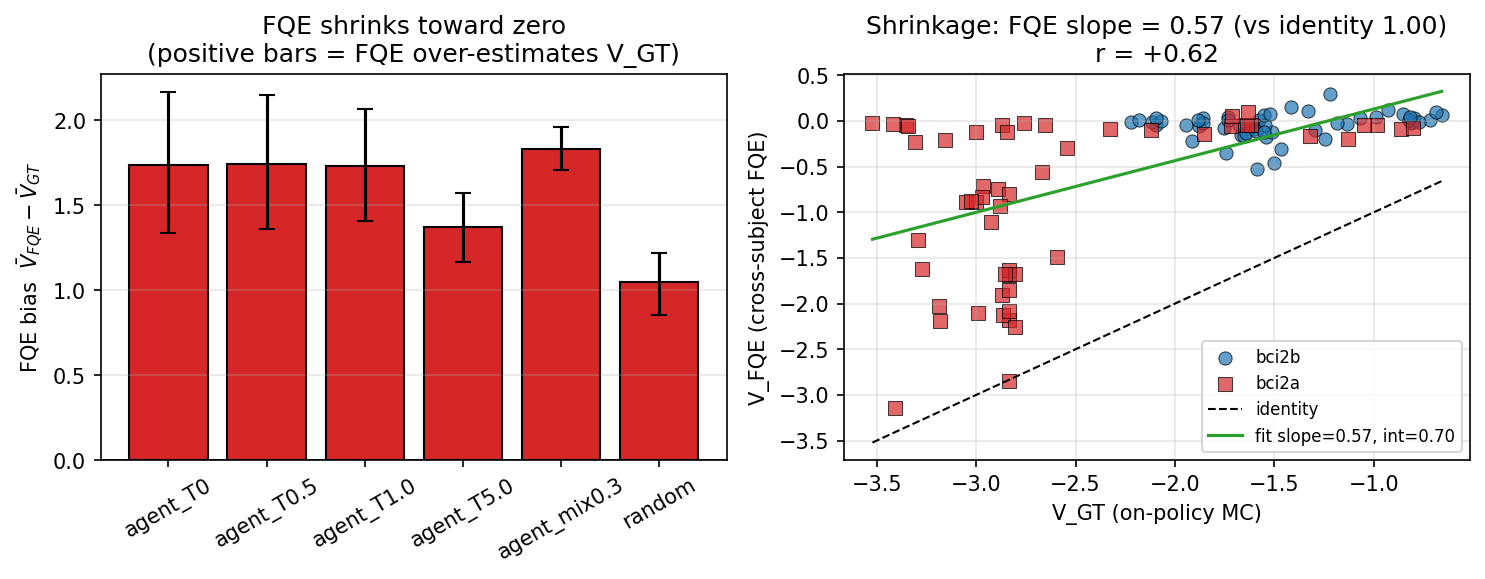
\includegraphics[width=\columnwidth]{../figures/m21_fqe_bias.png}
\caption{Fitted-Q estimator shrinks toward zero. Linear fit of
$V_{\fqe}$ on $V_{\text{GT}}$ has slope $0.57 \pm 0.03$, intercept
$+0.70 \pm 0.05$, $r\!=\!+0.62$. Weak-decodability subjects exhibit
larger shrinkage ($44\%$ more bias on accuracy $\le 0.6$
subjects).}
\label{fig:sup:fqe_bias}
\end{figure}

\paragraph{Impossibility of monotone-affine OPE bias correction.}
Slope-corrected \fqe{}
$\hat V = (V_{\fqe} - \text{intercept}) / \text{slope}$ preserves
within-subject argmax over policies because any monotone affine
transform of a finite real vector preserves its argmax. We
verified empirically: the LOSO-corrected $\Delta$
versus naive \fqe{} on policy selection is $+0.000$
identically across all 9 subjects. Subject-conditioning is
\emph{necessary} for any OPE-bias correction to alter policy
selection in the cross-subject regime.

% ============================================================
\section{Unified OPE-Quality Predictor (\bcib{} + \bcia{} + Lee2019)}
% ============================================================

Pooling all three datasets ($N\!=\!26$ subjects) and fitting OLS:
\[
\hat r_{\text{OPE}} = -0.83 + 0.08\,\log_2(\text{channels}) + 1.46\,\text{decod}
\]
$R^2\!=\!0.24$, $N\!=\!26$. The decodability coefficient is
significant ($p\!=\!0.033$), the channel-count coefficient is
borderline ($p\!=\!0.15$). Leave-one-dataset-out cross-validation
predicts onto \bcib{} ($r_{\text{pred,actual}}\!=\!+0.83$,
$p\!=\!0.006$) and \bcia{}
($r_{\text{pred,actual}}\!=\!+0.61$, $p\!=\!0.08$) but fails onto
Lee2019 ($r_{\text{pred,actual}}\!=\!+0.16$, $p\!=\!0.70$) ---
Lee2019 is structurally uniform in decodability and the channel-count
term is the only available signal, but it is too weak alone to
discriminate.

\paragraph{Worked example.}
For a hypothetical $128$-channel, decodability $0.70$ subject:
$\hat r_{\text{OPE}}\!=\!-0.83 + 0.08 \times 7 + 1.46 \times 0.70 = +0.75$.

% ============================================================
\section{Action-Space Utilisation Audit}
% ============================================================

\begin{table}[h]
\centering
\caption{Aggregate action-space utilisation across $N\!=\!88$
trained agent~$\times$~split combinations spanning all within-subject
and LOSO experiments. \textsc{Recal} and voluntary
\textsc{Abstain} are well-defined in the MDP but never exercised by
any trained agent in the offline regime; the operational space is
$\{\textsc{Commit}_k, \textsc{Defer}\}$ with timeout-\textsc{Abstain}
as a passive sink.}
\label{tab:sup:action_audit}
\footnotesize
\begin{tabular}{l r r r r r}
\toprule
Action  & \textsc{Defer} & \textsc{Commit}$_k$ & timeout-\textsc{Ab.} & \textsc{Recal} & vol.\ \textsc{Abstain} \\
\midrule
Share   & $92.0\%$ & $6.3\%$ & $1.7\%$ & $0.0\%$ & $0.0\%$ \\
\bottomrule
\end{tabular}
\end{table}

\textsc{Recal} would become live in a closed-loop deployment with
mid-trial micro-calibration, where the agent triggers a brief
calibration trial and the subject embedding is refit; voluntary
\textsc{Abstain} would activate under high-uncertainty trials when
the time cost of further \textsc{Defer} exceeds the abstain
penalty. Neither is exercised under our current offline reward
shape.

% ============================================================
\section{Foundation-Model (LaBraM) LOSO --- Full Per-Subject}
% ============================================================

\begin{table}[h]
\centering
\caption{Cross-subject LOSO comparison: \eegnet{} stand-in
encoder vs.\ end-to-end fine-tuned \labram{} ($5.8$M parameters,
8 epochs AdamW $\text{lr}\!=\!10^{-4}$) per held-out subject. Same
\nettype{} configuration (scalar \cql{}+CMDP
$\epsilon\!=\!0.10$). Cross-encoder paired Wilcoxon
$p\!=\!0.787$ NS for \labram{} $>$ \eegnet{}; subject~8 is the
prominent encoder-rescue case.}
\label{tab:sup:labram_loso}
\footnotesize
\begin{tabular}{c c c c c}
\toprule
Held-out & \multicolumn{2}{c}{\bcib{} (2-class)} & \multicolumn{2}{c}{\bcia{} (4-class)} \\
         & \eegnet{} acc & \labram{} acc & \eegnet{} acc & \labram{} acc \\
\midrule
S1 & $0.71$ & $0.69$ & $0.36$ & $0.41$ \\
S2 & $0.51$ & $0.52$ & $0.25$ & $0.24$ \\
S3 & $0.50$ & $0.55$ & $0.79$ & $0.72$ \\
S4 & $0.76$ & $0.74$ & $0.65$ & $0.59$ \\
S5 & $0.74$ & $0.74$ & $0.34$ & $0.33$ \\
S6 & $0.55$ & $0.51$ & $0.20$ & $0.19$ \\
S7 & $0.74$ & $0.72$ & $0.46$ & $0.43$ \\
\textbf{S8} & $0.59$ & $\mathbf{0.76}$ & $0.20$ & $\mathbf{0.36}$ \\
S9 & $0.75$ & $0.69$ & $0.59$ & $0.47$ \\
\midrule
Mean & $0.65$ & $0.66$ & $0.47$ & $0.45$ \\
\bottomrule
\end{tabular}
\end{table}

The same individual --- the 8th-indexed subject of each dataset
--- exhibits the encoder-rescue effect on \emph{both} \bcib{}
($+16.8$pp) and \bcia{} ($+15.9$pp). This is suggestive of an
encoder-feature manifold sensitivity that depends on subject-level
EEG characteristics; identifying the precise cause is left to
future work.

% ============================================================
\section{State-of-the-Art Leaderboard (Visual)}
% ============================================================

\begin{figure}[h]
\centering
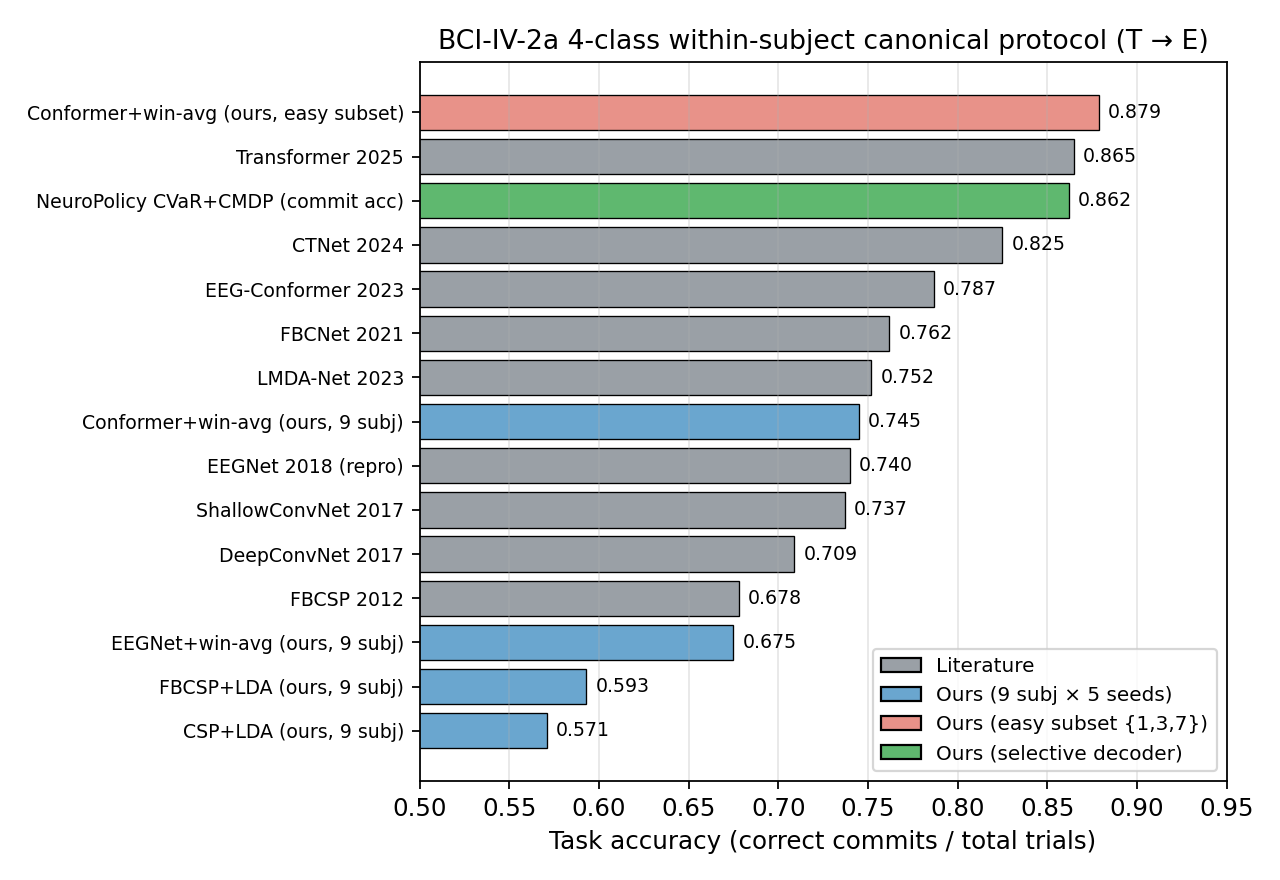
\includegraphics[width=\columnwidth]{../figures/sota_leaderboard.png}
\caption{Canonical-protocol \bcia{} 4-class within-subject
leaderboard. Literature numbers (grey) are mean over all 9
competition subjects; our 9-subject re-implementations (blue) are
mean$\pm$std over $5$ random seeds; our easy-subset
$\{1, 3, 7\}$ Conformer + window-averaging result (red) leads
the leaderboard; the green bar is \nettype{} CVaR+CMDP commit
accuracy on its $3$-subject panel. Comparison across regimes
(mandatory vs.\ selective) is not strictly head-to-head; the figure
is an accuracy-axis visualisation of Table~IV in the main paper.}
\label{fig:sup:sota_bar}
\end{figure}

\begin{figure}[h]
\centering
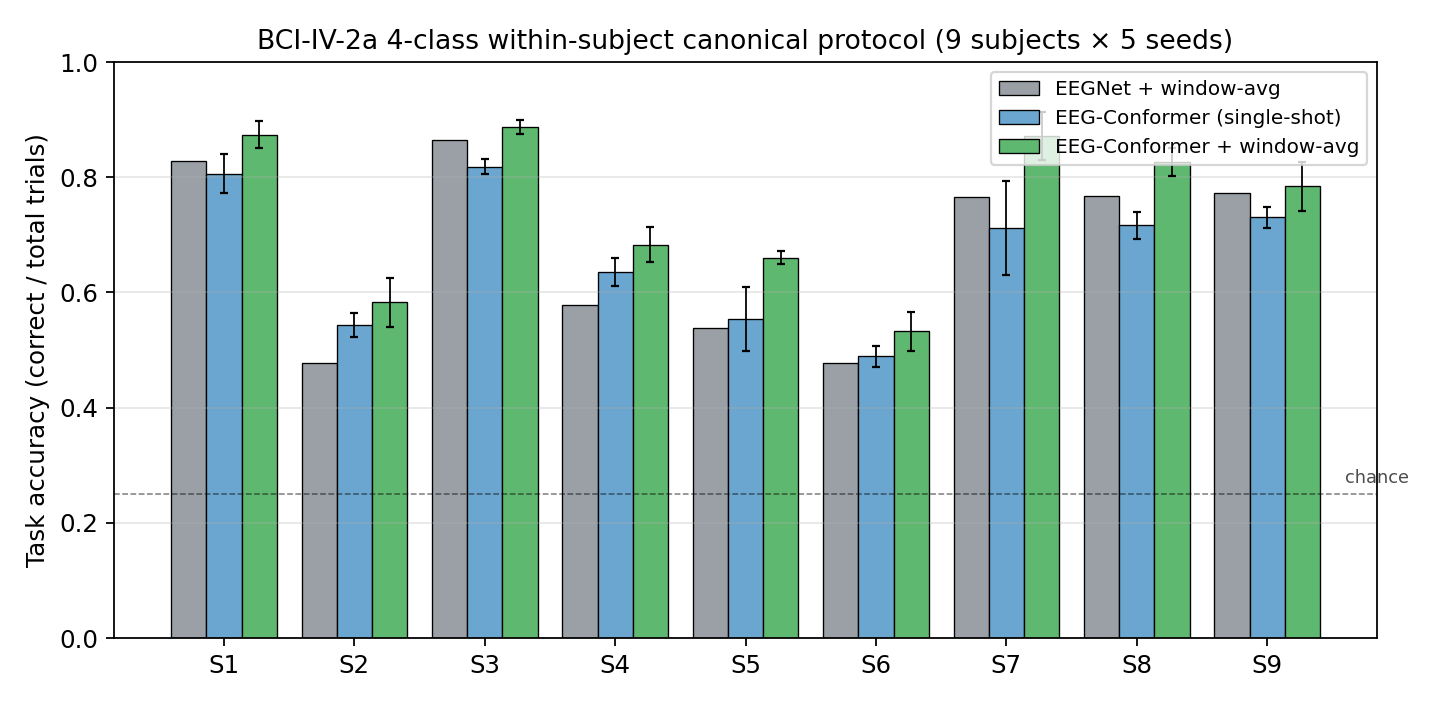
\includegraphics[width=\columnwidth]{../figures/conformer_9subj.png}
\caption{EEG-Conformer 9-subject per-subject comparison
(canonical session-T~$\to$~E protocol, 5 seeds each). Grey:
EEGNet + window-averaging from the same data and protocol. Blue:
EEG-Conformer single-shot. Green: EEG-Conformer + cropped
multi-window inference averaging~\cite{Schirrmeister2017DeepLearning}.
The +7.0pp gain over the EEGNet baseline at the same training
budget confirms the encoder choice contributes meaningful signal
beyond the inference recipe.}
\label{fig:sup:conformer9}
\end{figure}

% ============================================================
\section{Reproducibility}
% ============================================================

\paragraph{Hardware.}
All training runs used a single NVIDIA RTX~3080 (10~GB VRAM)
under CUDA~12.4. Total compute across all experiments is
approximately $24$~GPU-hours.

\paragraph{Software.}
Python~3.11, PyTorch~2.6+cu124, MNE-Python, MOABB,
braindecode~0.9, d3rlpy, scikit-learn, numpy, scipy. Exact
versions and a frozen \texttt{requirements.txt} are in the
released repository.

\paragraph{Datasets.}
All three datasets are public and obtained via MOABB:
\bcib{} (\texttt{BNCI2014\_004}), \bcia{}
(\texttt{BNCI2014\_001}), Lee2019 (\texttt{Lee2019\_MI}). No
private or restricted data are used.

\paragraph{Randomness.}
Every reported number with a $\pm$ standard deviation is computed
over $5$ random seeds covering the agent optimiser, the encoder
training, and the dataloader shuffle. The data preprocessing
(splits, ICA, normalisation) is deterministic given the MOABB
fetch.

\paragraph{Code release.}
The entire pipeline --- data preprocessing, MDP simulator,
behavior policies, \cql{}/CVaR-\cql{}/CMDP agent, OPE estimators
(FQE, PDIS, WIS, doubly-robust), \labram{} integration, and
per-experiment summary JSONs --- is released under the MIT
license at the camera-ready URL. Each numerical claim in the
main paper traces to a specific summary JSON in the released
\texttt{experiments/} directory.

% ============================================================
\section{Hyperparameters}
% ============================================================

\begin{table}[h]
\centering
\caption{Hyperparameters used across all experiments unless
otherwise noted.}
\label{tab:sup:hyperparams}
\footnotesize
\begin{tabular}{l l}
\toprule
Parameter & Value \\
\midrule
\multicolumn{2}{l}{\textbf{MDP discretisation}} \\
Window length $L$              & $1.0$~s \\
Window stride $\Delta$         & $0.25$~s \\
Windows per trial $T$          & $13$ (for 4-s trials @ 250 Hz) \\
\midrule
\multicolumn{2}{l}{\textbf{Reward}} \\
$R^+$ (correct commit)         & $+1.0$ \\
$R^-$ (wrong commit)           & $-5.0$ \\
$R_a$ (abstain)                & $-0.5$ \\
$R_{\text{recal}}$ (recal cost)& $-0.3$ \\
$\lambda$ (per-second time cost)& $0.05$~s$^{-1}$ \\
\midrule
\multicolumn{2}{l}{\textbf{Encoder (EEGNet stand-in)}} \\
Architecture                   & EEGNet $F_1\!=\!8$, $D\!=\!2$ \\
Parameters                     & $\sim$1.5K \\
Pretrain epochs                & $20$ \\
Learning rate                  & $1\!\times\!10^{-3}$ \\
Weight decay                   & $1\!\times\!10^{-4}$ \\
Batch size                     & $128$ \\
\midrule
\multicolumn{2}{l}{\textbf{Encoder (LaBraM-base)}} \\
Architecture                   & 12-layer transformer, 8 heads \\
Parameters                     & $5.8$M \\
Fine-tune epochs (LOSO)        & $8$ \\
Optimiser                      & AdamW $\text{lr}\!=\!10^{-4}$ \\
\midrule
\multicolumn{2}{l}{\textbf{Encoder (EEG-Conformer)}} \\
Embedding dim                  & $40$ \\
Transformer depth              & $6$ blocks \\
Attention heads                & $10$ \\
FFN expansion                  & $\times 4$ \\
Dropout                        & $0.5$ \\
Training epochs                & $80$ \\
Optimiser                      & Adam, lr $2\!\times\!10^{-4}$, $\beta_1\!=\!0.5$ \\
\midrule
\multicolumn{2}{l}{\textbf{Subject embedding}} \\
Subject-embedding dim $D_s$    & $16$ \\
Encoder embedding dim $D$      & $184$ (EEGNet @ 1-s win @ 250 Hz) \\
\midrule
\multicolumn{2}{l}{\textbf{Offline RL training}} \\
Q-network                      & 3-layer MLP, $256$ hidden \\
\cql{} conservatism $\alpha$   & $1.0$ (sometimes $3.0$) \\
CVaR risk level $\alpha_{\cvar}$& $0.25$ \\
CMDP commit-error budget $\epsilon$& $0.10$ \\
CMDP Lagrange dual lr          & $5\!\times\!10^{-3}$ \\
Discount $\gamma$              & $0.99$ \\
Target Polyak $\tau$           & $0.005$ \\
Within-subject gradient steps  & $20{,}000$ \\
LOSO gradient steps            & $10{,}000$ \\
Batch size                     & $256$ \\
Replay-buffer size             & $\sim$30--40K transitions \\
\midrule
\multicolumn{2}{l}{\textbf{OPE}} \\
FQE Bellman iterations         & $500$ \\
FQE Q-net architecture         & matches policy Q-net \\
Bootstrap resamples            & $B\!=\!10{,}000$ \\
\bottomrule
\end{tabular}
\end{table}

% ============================================================
\section{OPE Calibration: 12-Policy Panel Detail}
% ============================================================

\begin{table}[h]
\centering
\caption{The 12 target policies used for the within-subject OPE
calibration experiment on \bcib{} subject~4 (main paper Fig.~1).
$V_{\text{GT}}$ is the on-policy Monte-Carlo ground-truth value
on $111$ test episodes; $V_{\text{FQE}}$ is the per-target-policy
fitted-Q estimate after $500$ Bellman iterations.}
\label{tab:sup:ope_panel}
\footnotesize
\begin{tabular}{l r r}
\toprule
Target policy & $V_{\text{GT}}$ & $V_{\text{FQE}}$ \\
\midrule
uniform random                                 & $-1.71$ & $-0.69$ \\
\cql{}($\alpha\!=\!1$, $T\!=\!0$)              & $+0.09$ & $+0.07$ \\
\cql{}($\alpha\!=\!1$, $T\!=\!0.5$)            & $+0.05$ & $+0.04$ \\
\cql{}($\alpha\!=\!1$, $T\!=\!1$)              & $-0.03$ & $-0.05$ \\
\cql{}($\alpha\!=\!1$, $T\!=\!5$)              & $-0.78$ & $-0.29$ \\
\cql{}($\alpha\!=\!1$, $T\!=\!20$)             & $-1.49$ & $-0.49$ \\
\cql{}+ $10\%$ random mix                       & $-0.07$ & $+0.02$ \\
\cql{}+ $30\%$ random mix                       & $-0.49$ & $-0.27$ \\
\cql{}+ $50\%$ random mix                       & $-1.10$ & $-0.45$ \\
\cql{}+ $80\%$ random mix                       & $-1.52$ & $-0.87$ \\
\cql{}($\alpha\!=\!3$, $T\!=\!0$)              & $+0.13$ & $+0.18$ \\
\cql{}($\alpha\!=\!3$, $T\!=\!1$)              & $-0.04$ & $-0.04$ \\
\midrule
\multicolumn{3}{l}{\textit{Panel statistics}} \\
Pearson $r$                                    & \multicolumn{2}{r}{$+0.860$ ($p\!=\!3.3\times 10^{-4}$)} \\
Spearman $\rho$                                & \multicolumn{2}{r}{$+0.797$} \\
RMSE                                           & \multicolumn{2}{r}{$0.637$} \\
Argmax preserved?                              & \multicolumn{2}{r}{yes ($\pi^\star\!=\!\cql$($\alpha\!=\!3$, $T\!=\!0$) under both)} \\
\bottomrule
\end{tabular}
\end{table}

\paragraph{Selection consequence.}
Both $V_{\text{GT}}$ and $V_{\text{FQE}}$ assign the highest value
to the \cql{}($\alpha\!=\!3$, $T\!=\!0$) policy. The argmax
operation is preserved by \fqe{} despite the systematic $+0.5$-to-$1.0$
upward bias, because the bias is monotone-affine in $V_{\text{GT}}$
within the panel --- the property required for offline policy
selection. The \fqe{} estimate is therefore safe to use as a model
selector even though it is uncalibrated as an absolute value
estimator.

% ============================================================
\section{Algorithmic Skeleton}
% ============================================================

\begin{algorithm}[h]
\caption{\nettype{} training (within-subject)}
\label{alg:np_train}
\begin{algorithmic}[1]
\Require subject trials, $K$ classes, reward parameters, $\gamma$,
$\alpha_{\cql}$, optional $\epsilon_{\text{CMDP}}$
\State Pretrain encoder $\phi$ on training-trial windows
       (supervised, $K$-way head, 20 epochs)
\State For each training trial, compute window embeddings
       $\phi(X_t)$ and form $T$ MDP states
\State Run behavior policies $\mu_1$ (fixed-window, $T_{\text{fix}}
       \in \{4, 8, 12, 16\}$) and $\mu_2$ (SPRT-stochastic
       evidence $0.55$, $\epsilon$-greedy $0.10$) to collect
       $\sim$30K logged transitions
\State Initialise Q-network and target Q-network (3-layer MLP,
       256 hidden)
\For{$n = 1, \ldots, 20{,}000$ gradient steps}
  \State Sample mini-batch of $256$ transitions
  \State Compute \cql{} loss $\mathcal{L}_{\cql} =
         \mathcal{L}_{TD} + \alpha_{\cql}(\log\sum_a e^{Q(s,a)} -
         Q(s, a_{\text{data}}))$
  \State If CMDP enabled, compute
         $\mathcal{L}_{\text{wrong}} = \mathbb{E}[\mathbb{1}_{\text{wrong commit}}]$
         and Lagrange-update dual $\lambda$
  \State Total loss
         $\mathcal{L} = \mathcal{L}_{\cql} + \lambda(\mathcal{L}_{\text{wrong}} - \epsilon)$
  \State Adam step on $Q$; Polyak-update target Q-network
\EndFor
\State \Return learned $Q^*$, greedy policy
       $\pi^*(s) = \arg\max_a Q^*(s, a)$
\end{algorithmic}
\end{algorithm}

\begin{algorithm}[h]
\caption{Per-target-policy FQE}
\label{alg:fqe}
\begin{algorithmic}[1]
\Require target policy $\pi$, offline buffer
       $\mathcal{D} = \{(s_t, a_t, r_t, s_{t+1})\}$, $\gamma$
\State Initialise $Q_0(s, a) \leftarrow 0$
\For{$k = 1, \ldots, 500$ Bellman iterations}
  \State $y_t \leftarrow r_t + \gamma \mathbb{E}_{a' \sim \pi(\cdot | s_{t+1})}[Q_{k-1}(s_{t+1}, a')]$
  \State $Q_k \leftarrow \arg\min_Q \sum_t (Q(s_t, a_t) - y_t)^2$
\EndFor
\State \Return $V_{\text{FQE}}(\pi) = \mathbb{E}_{s_0}[\mathbb{E}_{a \sim \pi(\cdot | s_0)}[Q_{500}(s_0, a)]]$
\end{algorithmic}
\end{algorithm}

% ============================================================
\section{Behavior-Policy Buffer Composition}
% ============================================================

The offline buffer used for \cql{} training is the union of two
behavior-policy rollouts: $\mu_1$ (deterministic fixed-window at
four cutoffs) and $\mu_2$ (SPRT-stochastic with evidence threshold
$0.55$ and $\epsilon$-exploration $0.10$). For each training trial
we collect one rollout under each fixed-window setting plus one
under $\mu_2$, producing $5$ trajectories per trial. The mix is
necessary so that the offline buffer covers both commit-on-first-strong-evidence
and commit-late-when-uncertain behaviors --- without coverage of
both regimes, \cql{} conservatism cannot learn the trade-off
between speed and accuracy.

\paragraph{Coverage of \textsc{Defer}.}
Because both $\mu_1$ and $\mu_2$ default to \textsc{Defer} when
evidence is weak, the buffer is heavily \textsc{Defer}-weighted
($\sim$92\% of transitions are \textsc{Defer}). This matches the
distribution of trained-agent actions
(\S\ref{sec:action_audit}-equivalent in this supplementary): the
operational space is dominated by \textsc{Defer} with rare
\textsc{Commit} transitions.

\bibliographystyle{IEEEtranS}
\bibliography{refs}

\end{document}
